\hypertarget{RandomForest_8c}{
\section{Random\-Forest.c File Reference}
\label{RandomForest_8c}\index{RandomForest.c@{RandomForest.c}}
}
{\tt \#include \char`\"{}party.h\char`\"{}}\par


Include dependency graph for Random\-Forest.c:\begin{figure}[H]
\begin{center}
\leavevmode
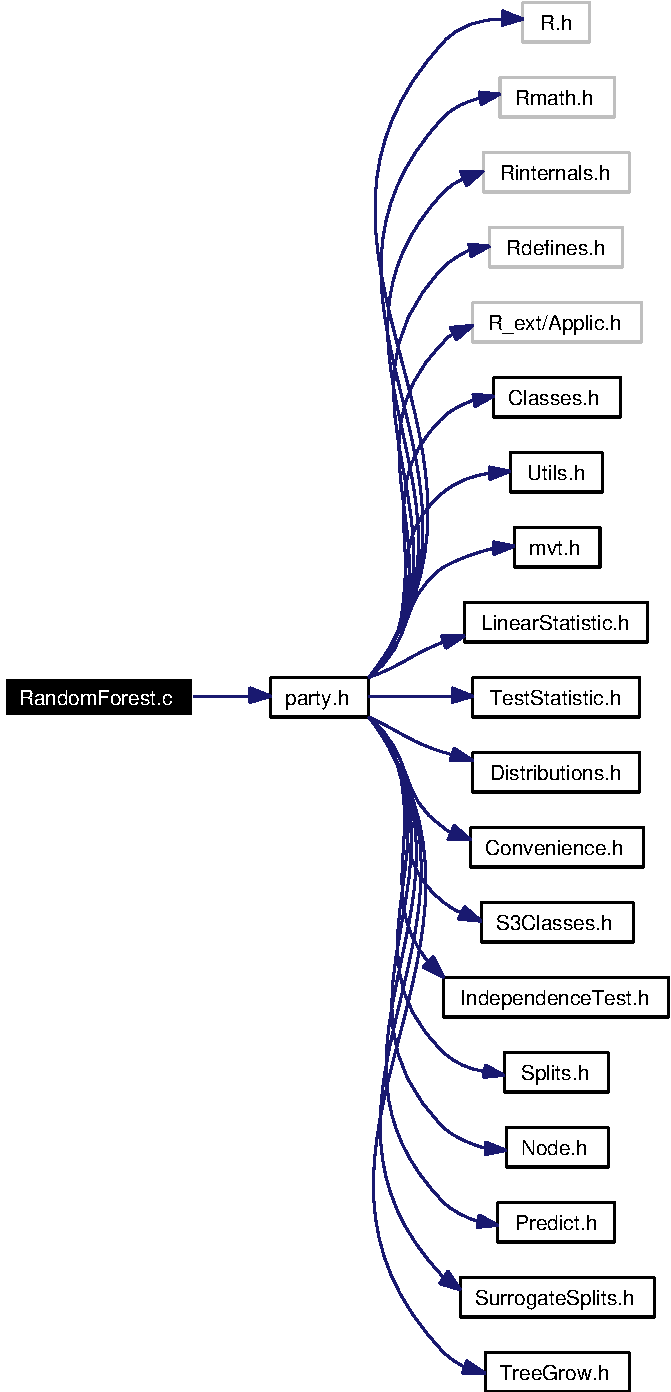
\includegraphics[width=178pt]{RandomForest_8c__incl}
\end{center}
\end{figure}
\subsection*{Functions}
\begin{CompactItemize}
\item 
SEXP \hyperlink{RandomForest_8c_1d975bfdaf516bceb762e16659920f8a}{R\_\-Ensemble} (SEXP learnsample, SEXP weights, SEXP fitmem, SEXP controls)
\end{CompactItemize}


\subsection{Detailed Description}
Random forest with conditional inference trees

\begin{Desc}
\item[Author:]\begin{Desc}
\item[Author]hothorn \end{Desc}
\end{Desc}
\begin{Desc}
\item[Date:]\begin{Desc}
\item[Date]2007-02-02 11:22:45 +0100 (Fri, 02 Feb 2007) \end{Desc}
\end{Desc}


Definition in file \hyperlink{RandomForest_8c-source}{Random\-Forest.c}.

\subsection{Function Documentation}
\hypertarget{RandomForest_8c_1d975bfdaf516bceb762e16659920f8a}{
\index{RandomForest.c@{Random\-Forest.c}!R_Ensemble@{R\_\-Ensemble}}
\index{R_Ensemble@{R\_\-Ensemble}!RandomForest.c@{Random\-Forest.c}}
\subsubsection[R\_\-Ensemble]{\setlength{\rightskip}{0pt plus 5cm}SEXP R\_\-Ensemble (SEXP {\em learnsample}, SEXP {\em weights}, SEXP {\em fitmem}, SEXP {\em controls})}}
\label{RandomForest_8c_1d975bfdaf516bceb762e16659920f8a}


An experimental implementation of random forest like algorithms \par
 \begin{Desc}
\item[Parameters:]
\begin{description}
\item[{\em learnsample}]an object of class `Learning\-Sample' \item[{\em weights}]a vector of case weights \item[{\em fitmem}]an object of class `Tree\-Fit\-Memory' \item[{\em controls}]an object of class `Tree\-Control' \end{description}
\end{Desc}


Definition at line 21 of file Random\-Forest.c.

References C\_\-init\_\-node(), C\_\-Sample\-No\-Replace(), get\_\-fraction(), get\_\-maxsurrogate(), get\_\-ninputs(), get\_\-nobs(), get\_\-ntree(), get\_\-predict\_\-trafo(), get\_\-replace(), get\_\-splitctrl(), ncol(), NODE\_\-LENGTH, and PL2\_\-responses\-Sym.

Here is the call graph for this function:\begin{figure}[H]
\begin{center}
\leavevmode
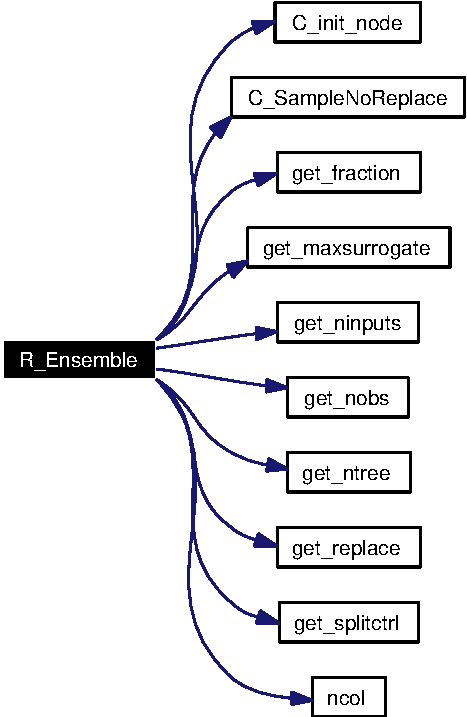
\includegraphics[width=129pt]{RandomForest_8c_1d975bfdaf516bceb762e16659920f8a_cgraph}
\end{center}
\end{figure}
